\documentclass[tikz,border=10pt]{standalone}
\usepackage{tikz}
\usetikzlibrary{shapes.geometric, arrows.meta, positioning, calc, fit, backgrounds}
\usepackage{amsmath,amssymb}
\usepackage{xcolor}

% Unified Academic Color Palette
\definecolor{cInput}{RGB}{235, 248, 255}
\definecolor{bInput}{RGB}{49, 130, 206}

\definecolor{cTrans}{RGB}{240, 249, 255}
\definecolor{bTrans}{RGB}{43, 108, 176}

\definecolor{cGCN}{RGB}{230, 255, 250}
\definecolor{bGCN}{RGB}{49, 151, 149}

\definecolor{cRecurr}{RGB}{250, 245, 255}
\definecolor{bRecurr}{RGB}{128, 90, 213}

\definecolor{cHead}{RGB}{255, 245, 245}
\definecolor{bHead}{RGB}{229, 62, 62}

\definecolor{cFusion}{RGB}{254, 252, 191}
\definecolor{bFusion}{RGB}{214, 158, 46}

\definecolor{cGray}{RGB}{247, 250, 252}
\definecolor{bGray}{RGB}{160, 174, 192}

\definecolor{tDark}{RGB}{26, 32, 44}
\definecolor{tMuted}{RGB}{74, 85, 104}

\begin{document}
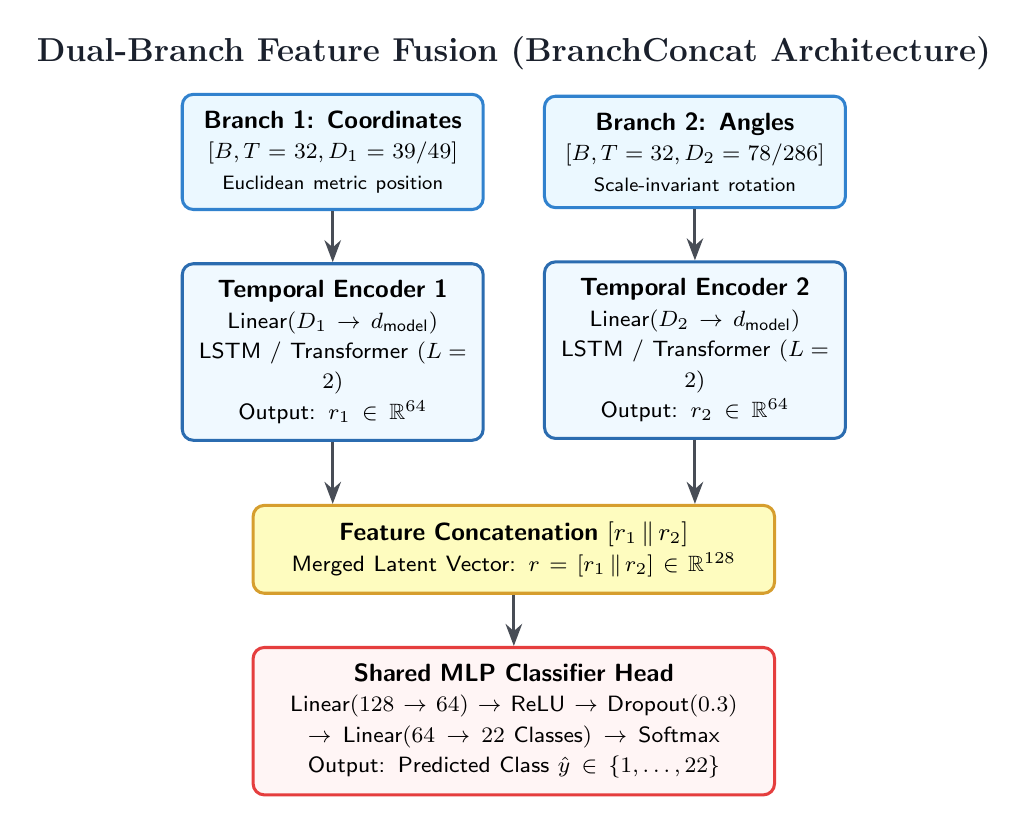
\begin{tikzpicture}[
    font=\sffamily\small,
    >=Stealth,
    node distance=0.65cm,
    block/.style={
        draw=#1,
        line width=1.1pt,
        rounded corners=4pt,
        align=center,
        inner sep=6pt
    },
    arrow/.style={->, line width=1.1pt, color=tDark!80}
]

\node[font=\bfseries\large, text=tDark] (title) at (3.8, 1.25) {Dual-Branch Feature Fusion (BranchConcat Architecture)};

% Branch 1: Coordinates
\node[block=bInput, fill=cInput, text width=3.4cm] (in1) at (1.5, 0) {
    \textbf{Branch 1: Coordinates}\\
    {\footnotesize $[B, T=32, D_1=39/49]$}\\
    {\scriptsize Euclidean metric position}
};

\node[block=bTrans, fill=cTrans, text width=3.4cm, below=of in1] (enc1) {
    \textbf{Temporal Encoder 1}\\
    {\footnotesize $\text{Linear}(D_1 \to d_{\text{model}})$}\\
    {\footnotesize $\text{LSTM / Transformer} \ (L=2)$}\\
    {\footnotesize Output: $r_1 \in \mathbb{R}^{64}$}
};

% Branch 2: Angles
\node[block=bInput, fill=cInput, text width=3.4cm] (in2) at (6.1, 0) {
    \textbf{Branch 2: Angles}\\
    {\footnotesize $[B, T=32, D_2=78/286]$}\\
    {\scriptsize Scale-invariant rotation}
};

\node[block=bTrans, fill=cTrans, text width=3.4cm, below=of in2] (enc2) {
    \textbf{Temporal Encoder 2}\\
    {\footnotesize $\text{Linear}(D_2 \to d_{\text{model}})$}\\
    {\footnotesize $\text{LSTM / Transformer} \ (L=2)$}\\
    {\footnotesize Output: $r_2 \in \mathbb{R}^{64}$}
};

\draw[arrow] (in1) -- (enc1);
\draw[arrow] (in2) -- (enc2);

% Merge
\node[block=bFusion, fill=cFusion, text width=6.2cm, below=0.8cm of $(enc1.south)!0.5!(enc2.south)$] (concat) {
    \textbf{Feature Concatenation $[r_1 \,\|\, r_2]$}\\
    {\footnotesize Merged Latent Vector: $r = [r_1 \,\|\, r_2] \in \mathbb{R}^{128}$}
};

\node[block=bHead, fill=cHead, text width=6.2cm, below=of concat] (head) {
    \textbf{Shared MLP Classifier Head}\\
    {\footnotesize $\text{Linear}(128 \to 64) \to \text{ReLU} \to \text{Dropout}(0.3)$}\\
    {\footnotesize $\to \text{Linear}(64 \to 22 \text{ Classes}) \to \text{Softmax}$}\\
    {\footnotesize Output: Predicted Class $\hat{y} \in \{1, \dots, 22\}$}
};

\draw[arrow] (enc1.south) -- (concat.north -| enc1.south);
\draw[arrow] (enc2.south) -- (concat.north -| enc2.south);
\draw[arrow] (concat) -- (head);

\end{tikzpicture}
\end{document}
